\documentclass{article}[]
\newcommand{\ImageWidth}{11cm}
\usepackage{tikz}
\usetikzlibrary{decorations.pathreplacing,positioning, arrows.meta}

\usepackage{multirow}
\usepackage{graphicx}
\usepackage{float}


\usepackage{amsmath} % for \text
\tikzset{>=latex} % for LaTeX arrow head
\usepackage{xcolor}
\colorlet{myblue}{black!40!blue}
\colorlet{myred}{black!40!red}

\usepackage{dcolumn}

\begin{document}         
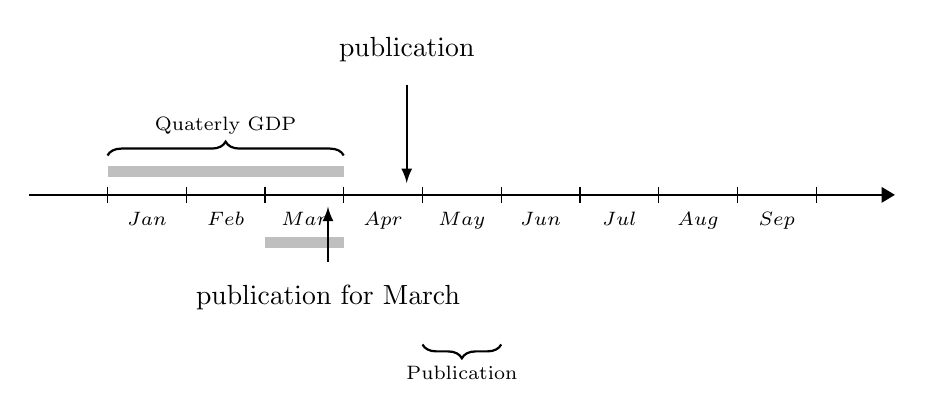
\begin{tikzpicture}
% draw horizontal line   
\draw[thick, -Triangle] (0,0) -- (\ImageWidth,0) node[font=\scriptsize,below left=3pt and -8pt]{ };

% draw vertical lines
\foreach \x in {1,...,10}
\draw (\x cm,3pt) -- (\x cm,-3pt);

\foreach \x/\descr in {1.5/Jan, 2.5/Feb, 3.5/Mar, 4.5/Apr, 5.5/May, 6.5/Jun, 7.5/Jul, 8.5/Aug,9.5/Sep}
\node[font=\scriptsize, text height=1.75ex,
text depth=.5ex] at (\x,-.3) {$\descr$};

% colored bar up
\foreach \x/\perccol in
{1/100,2/75,3/25}
\draw[lightgray, line width=4pt] 
(\x,.3) -- +(1,0);

% colored bar down
\foreach \x/\perccol in
{3/25}
\draw[lightgray, line width=4pt] 
(\x,-.6) -- +(1,0);


% braces
\draw [thick ,decorate,decoration={brace,amplitude=5pt}] (1,0.5)  -- +(3,0) 
       node [black,midway,above=4pt, font=\scriptsize] {Quaterly GDP};
\draw [thick,decorate,decoration={brace,amplitude=5pt}] (6,-1.9) -- +(-1,0)
      node [black,midway,font=\scriptsize, below=4pt] {Publication};

% time of publication
\node[align=center] at (4.8,1.85) {publication};
\draw [thick,->] (4.8,1.4) -- (4.8,0.15);
\node[align=center] at (3.8,-1.3) {publication for March};
\draw [thick,->] (3.8,-0.85) -- (3.8,-0.15);
\end{tikzpicture}


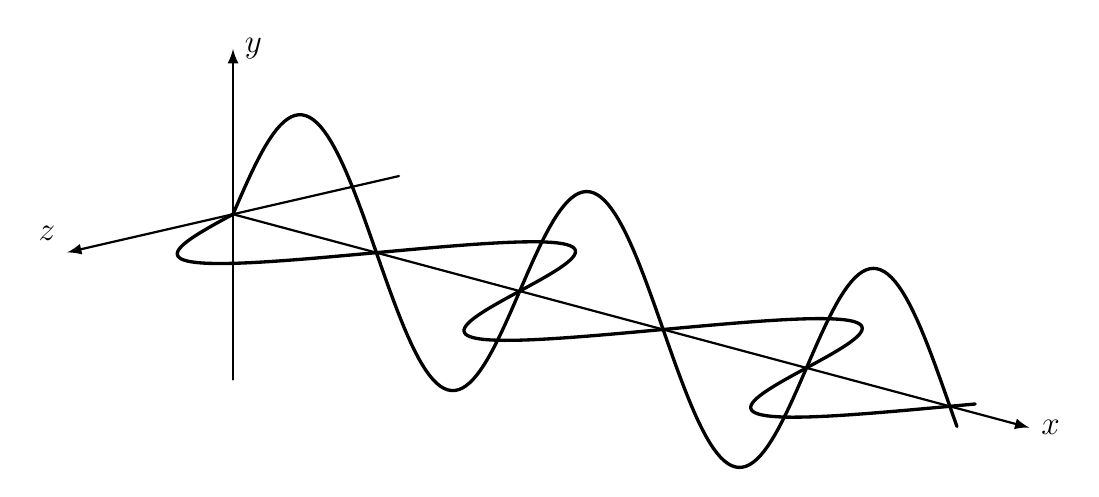
\begin{tikzpicture}[x=(-15:1.2), y=(90:1.0), z=(-150:1.0),
                    line cap=round, line join=round,
                    axis/.style={black, thick,->},
                    vector/.style={>=stealth,->}]
  \large
  \def\A{1.5}
  \def\nNodes{5} % use even number
  \def\nVectorsPerNode{8}
  \def\N{\nNodes*40}
  \def\xmax{\nNodes*pi/2*1.01}
  \pgfmathsetmacro\nVectors{(\nVectorsPerNode+1)*\nNodes}
 
  \def\vE{\mathbf{E}}
  \def\vB{\mathbf{B}}
  \def\vk{\mathbf{\hat{k}}}
 
  \draw[very thick,variable=\t,domain=0:\nNodes*pi/2*1.01,samples=\N]
    plot (\t,{\A*sin(\t*360/pi)},0);
  \draw[very thick,variable=\t,domain=0:\nNodes*pi/2*1.01,samples=\N]
    plot (\t,0,{\A*sin(\t*360/pi)});
 
  % main axes
  \draw[axis] (0,0,0) -- ++(\xmax*1.1,0,0) node[right] {$x$};
  \draw[axis] (0,-\A*1.4,0) -- (0,\A*1.4,0) node[right] {$y$};
  \draw[axis] (0,0,-\A*1.4) -- (0,0,\A*1.4) node[above left] {$z$};
 
  % ...
 
\end{tikzpicture}



% Electromagnetic wave - colored
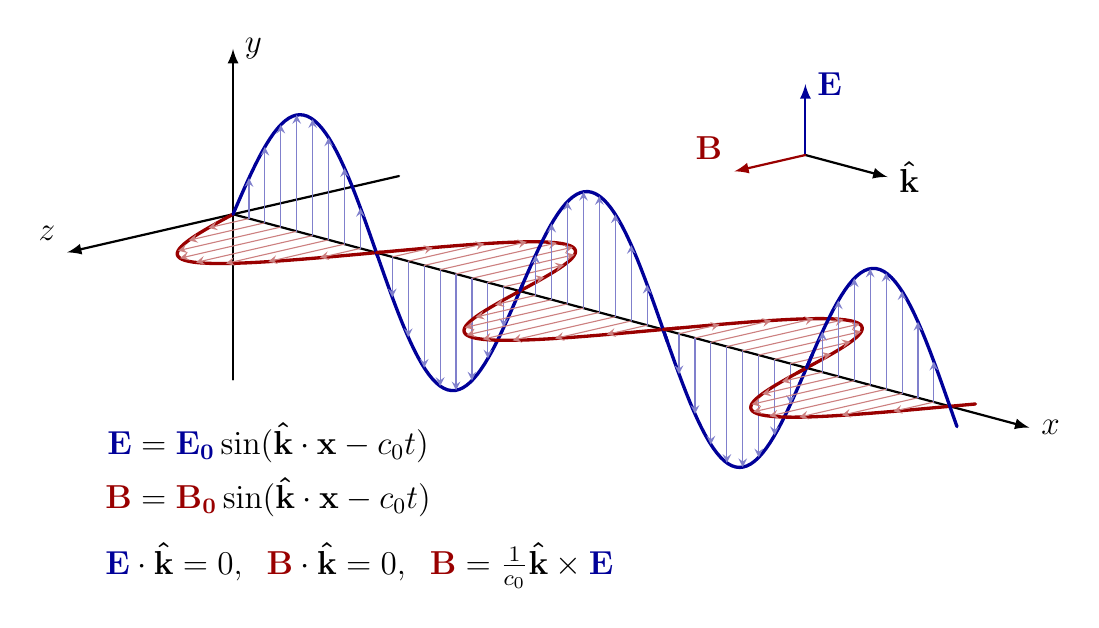
\begin{tikzpicture}[x=(-15:1.2), y=(90:1.0), z=(-150:1.0),
                    line cap=round, line join=round,
                    axis/.style={black, thick,->},
                    vector/.style={>=stealth,->}]
  \large
  \def\A{1.5}
  \def\nNodes{5} % use even number
  \def\nVectorsPerNode{8}
  \def\N{\nNodes*40}
  \def\xmax{\nNodes*pi/2*1.01}
  \pgfmathsetmacro\nVectors{(\nVectorsPerNode+1)*\nNodes}
 
  \def\vE{{\color{myblue}\mathbf{E}}}
  \def\vB{{\color{myred}\mathbf{B}}}
  \def\vk{\mathbf{\hat{k}}}
 
  \def\drawENode{ % draw E node and vectors with some offset
    \draw[myblue,very thick,variable=\t,domain=\iOffset*pi/2:(\iOffset+1)*pi/2*1.01,samples=40]
      plot (\t,{\A*sin(\t*360/pi)},0);
    \foreach \k [evaluate={\t=\k*pi/2/(\nVectorsPerNode+1);
                           \angle=\k*90/(\nVectorsPerNode+1);}]
                in {1,...,\nVectorsPerNode}{
      \draw[vector,myblue!50]  (\iOffset*pi/2+\t,0,0) -- ++(0,{\A*sin(2*\angle+\iOffset*180)},0);
    }
  }
  \def\drawBNode{ % draw B node and vectors with some offset
    \draw[myred,very thick,variable=\t,domain=\iOffset*pi/2:(\iOffset+1)*pi/2*1.01,samples=40]
      plot (\t,0,{\A*sin(\t*360/pi)});
    \foreach \k [evaluate={\t=\k*pi/2/(\nVectorsPerNode+1);
                           \angle=\k*90/(\nVectorsPerNode+1);}]
                in {1,...,\nVectorsPerNode}{
      \draw[vector,myred!50]  (\iOffset*pi/2+\t,0,0) -- ++(0,0,{\A*sin(2*\angle+\iOffset*180)});
    }
  }
 
  % main axes
  \draw[axis] (0,0,0) -- ++(\xmax*1.1,0,0) node[right] {$x$};
  \draw[axis] (0,-\A*1.4,0) -- (0,\A*1.4,0) node[right] {$y$};
  \draw[axis] (0,0,-\A*1.4) -- (0,0,\A*1.4) node[above left] {$z$};
 
  % small axes
  \def\xOffset{{(\nNodes-2)*pi/2}}
  \def\yOffset{\A*1.2}
  \def\zOffset{\A*1.2}
  \draw[axis,black] (\xOffset,\yOffset,-\zOffset) -- ++(\A*0.6,0,0) node[right,align=center] {$\mathbf{\hat{k}}$}; %\\propagation
  \draw[axis,myblue]  (\xOffset,\yOffset,-\zOffset) -- ++(0,\A*0.6,0) node[right] {$\mathbf{E}$};
  \draw[axis,myred]   (\xOffset,\yOffset,-\zOffset) -- ++(0,0,\A*0.6) node[above left] {$\mathbf{B}$};
 
  % equation
  \node[above right] at (\xOffset,-0.5*\yOffset,4*\zOffset)
    {$\begin{aligned}
      \vE &= {\color{myblue}\mathbf{E_0}}\sin(\vk\cdot\mathbf{x}-c_0t)\\
      \vB &= {\color{myred} \mathbf{B_0}}\sin(\vk\cdot\mathbf{x}-c_0t)\\
      \end{aligned}$};
  \node[below right] at (\xOffset,-0.5*\yOffset,4*\zOffset)
    {$\vE\cdot\vk = 0,\;\; \vB\cdot\vk = 0,\;\; \vB = \frac{1}{c_0}\vk\times\vE$};
 
  % draw (anti-)nodes
  \foreach \iNode [evaluate={\iOffset=\iNode-1;}] in {1,...,\nNodes}{
    \ifodd\iNode \drawBNode \drawENode % E overlaps B
    \else        \drawENode \drawBNode % B overlaps E
    \fi
  }
 
\end{tikzpicture}


\newpage

\begin{table}[!htbp] \centering 
  \caption{} 
  \label{} 
\begin{tabular}{@{\extracolsep{5pt}}lD{.}{.}{-3} D{.}{.}{-3} D{.}{.}{-3} D{.}{.}{-3} } 
\\[-1.8ex]\hline 
\hline \\[-1.8ex] 
 & \multicolumn{4}{c}{Linear Regression} \\ 
\cline{2-5} 
\\[-1.8ex] & \multicolumn{4}{c}{Year on Year GDP (in \%)} \\ 
\\[-1.8ex] & \multicolumn{1}{c}{(1)} & \multicolumn{1}{c}{(2)} & \multicolumn{1}{c}{(3)} & \multicolumn{1}{c}{(4)}\\ 
\hline \\[-1.8ex] 
 Constant & 3.434^{***} & 1.102^{***} & -0.920 & -1.403^{*} \\ 
  & (0.170) & (0.254) & (0.589) & (0.725) \\ 
  & & & & \\ 
 3 months lag of YoY GDP &  & 0.693^{***} & 0.575^{***} &  \\ 
  &  & (0.065) & (0.070) &  \\ 
  & & & & \\ 
 BSI & 14.867^{***} & 4.834^{***} & 9.064^{***} & 19.938^{***} \\ 
  & (1.351) & (1.367) & (1.717) & (1.373) \\ 
  & & & & \\ 
 Variance &  &  & 22.630^{***} & 45.301^{***} \\ 
  &  &  & (6.016) & (6.652) \\ 
  & & & & \\ 
\hline \\[-1.8ex] 
Observations & \multicolumn{1}{c}{124} & \multicolumn{1}{c}{123} & \multicolumn{1}{c}{123} & \multicolumn{1}{c}{124} \\ 
R$^{2}$ & \multicolumn{1}{c}{0.498} & \multicolumn{1}{c}{0.742} & \multicolumn{1}{c}{0.770} & \multicolumn{1}{c}{0.637} \\ 
Adjusted R$^{2}$ & \multicolumn{1}{c}{0.494} & \multicolumn{1}{c}{0.738} & \multicolumn{1}{c}{0.764} & \multicolumn{1}{c}{0.631} \\ 
Residual Std. Error & \multicolumn{1}{c}{1.174} & \multicolumn{1}{c}{0.848} & \multicolumn{1}{c}{0.805} & \multicolumn{1}{c}{1.002} \\ 
F Statistic & \multicolumn{1}{c}{121.091$^{***}$} & \multicolumn{1}{c}{172.776$^{***}$} & \multicolumn{1}{c}{132.525$^{***}$} & \multicolumn{1}{c}{106.248$^{***}$} \\ 
\hline 
\hline \\[-1.8ex] 
\textit{Note:}  & \multicolumn{4}{r}{$^{*}$p$<$0.1; $^{**}$p$<$0.05; $^{***}$p$<$0.01} \\ 
\end{tabular} 
\end{table} 


\newpage

\begin{tikzpicture}
\begin{axis}[
    domain=0:6*pi,
    samples=100,
    axis lines*=left, 
    axis line style={->},
    xtick={2.2, 4.5, 8.1}, ytick=\empty,
    xticklabels = {$Peak$, $Peak$, $Peak$},
    width=14cm, height=8cm,
    xlabel={time}, ylabel={GDP}
]       
\addplot[mark=none, dashed] coordinates {(2.2, -1) (2.2, 4)};
\addplot[mark=none, dashed] coordinates {(4.5, -1) (4.5, 1)}; 
\addplot[mark=none, dashed] coordinates {(8.1, -1) (8.1, 12)}; %\addplot [thick, gray] {x};
\addplot [thick, black] {x + 4*sin(deg(x)) * sin(deg(x/6))^0.5}
%    node [pos=0.1, anchor=south] {Peak}
    node [pos=0.3, anchor=south, sloped] {Expansion}
    node [pos=0.49, anchor=south, sloped] {Recession}
% Add line to show end of and ... peak and ... line
;
\end{axis}
\end{tikzpicture}

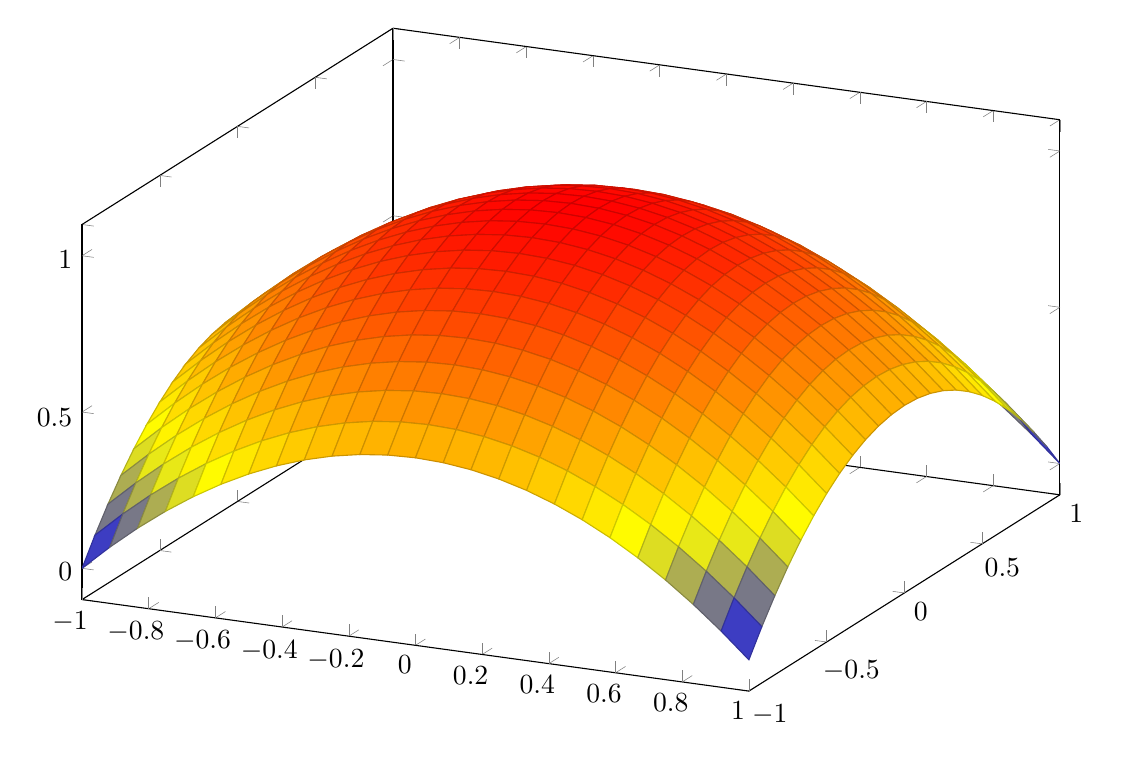
\begin{tikzpicture}
\begin{axis}[domain=-1:1,
    width=14cm, height=10cm]
\addplot3[
    surf,
]
{((1 - x^2) + (1 - y^2))/2};

\end{axis}
\end{tikzpicture}



\begin{tikzpicture}
    \begin{axis}[
      ybar,
      bar width=40pt,
      xlabel={Answers},
      ylabel={Proportion},
      ymin=0,
      ytick=\empty, xtick=data,
      axis x line=bottom,
      axis y line=left,
      enlarge x limits=1,
      symbolic x coords={negative,neutral,positive},
      xticklabel style={anchor=base,yshift=-\baselineskip},
      nodes near coords={\pgfmathprintnumber\pgfplotspointmeta\%},
        width=14.8cm, height=8cm
    ]
      \addplot[fill=white] coordinates {
        (negative,30)
        (neutral,50)
        (positive,20)
      };
    \end{axis}

    \begin{axis}[every axis plot post/.append style={
        mark=none,domain=-3:3,samples=50,smooth}, % All plots: from -2:2, 50 samples, smooth, no marks
          axis x line*=bottom, % no box around the plot, only x and y axis
          axis y line*=left, % the * suppresses the arrow tips
          xtick=\empty, ytick=\empty,
          width=16cm, height=8cm,
          enlargelimits=upper] % extend the axes a bit to the right and top
          \addplot {gauss(0,0.5)};
          \addplot {gauss(0,1)};
        %  \addplot [ybar, bar width=5pt] coordinates { (-1, 1) (0, 3)};
    \end{axis}
\end{tikzpicture}


\begin{figure}
    \centering
\begin{tikzpicture}
    \begin{axis}[every axis plot post/.append style={
        mark=none,domain=-3:3,samples=50,smooth}, % All plots: from -2:2, 50 samples, smooth, no marks
          axis x line*=bottom, % no box around the plot, only x and y axis
          axis y line*=left, % the * suppresses the arrow tips
          xtick=\empty, ytick=\empty,
          width=10cm, height=4cm,
          enlargelimits=upper] % extend the axes a bit to the right and top
          \addplot {gauss(0,0.5)};
          \addplot {gauss(0,1)};
        %  \addplot [ybar, bar width=5pt] coordinates { (-1, 1) (0, 3)};
    \end{axis}
\end{tikzpicture}
    \caption{The Variance}
    \label{fig:var_explanation}
\end{figure}

\begin{figure}
    \centering
  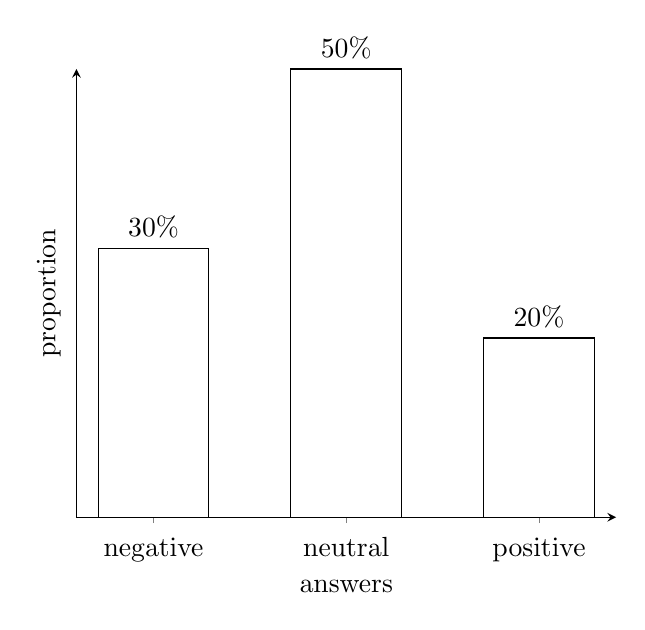
\begin{tikzpicture} %[font=\small]
    \begin{axis}[
      ybar,
      bar width=40pt,
      xlabel={answers},
      ylabel={proportion},
      ymin=0,
      ytick=\empty,
      xtick=data,
      axis x line=bottom,
      axis y line=left,
      enlarge x limits=0.2,
      symbolic x coords={negative,neutral,positive},
      xticklabel style={anchor=base,yshift=-\baselineskip},
      nodes near coords={\pgfmathprintnumber\pgfplotspointmeta\%}
    ]
      \addplot[fill=white] coordinates {
        (negative,30)
        (neutral,50)
        (positive,20)
      };
    \end{axis}
  \end{tikzpicture}
    \caption{Caption}
    \label{fig:hist_example}
\end{figure}


\newpage

\begin{table}[!htbp] \centering 
%  \caption{} 
  \label{tab:model} 
\begin{tabular}{@{\extracolsep{5pt}}lD{.}{.}{-3} D{.}{.}{-3} D{.}{.}{-3} D{.}{.}{-3} } 
\\[-1.8ex]\hline 
\hline \\[-1.8ex] 
 & \multicolumn{4}{c}{Linear Regression} \\ 
\cline{2-5} 
\\[-1.8ex] & \multicolumn{4}{c}{Year on Year GDP (in \%)} \\ 
\\[-1.8ex] & \multicolumn{1}{c}{(1)} & \multicolumn{1}{c}{(2)} & \multicolumn{1}{c}{(3)} & \multicolumn{1}{c}{(4)}\\ 
\hline \\[-1.8ex] 
 Constant & 3.434^{***} & 1.114^{***} & -1.829^{**} & -4.052^{***} \\ 
  & (0.170) & (0.255) & (0.867) & (0.922) \\ 
  &&&& \\ 
 3 months lag of YoY GDP &  & 0.690^{***} & 0.525^{***} &  \\ 
  &  & (0.066) & (0.078) &  \\ 
  &&&& \\ 
 BSI & 15.053^{***} & 4.957^{***} & 10.621^{***} & 22.080^{***} \\ 
  & (1.364) & (1.387) & (2.079) & (1.392) \\ 
  &&&& \\ 
 Variance &  &  & 12.831^{***} & 27.506^{***} \\ 
  &  &  & (3.628) & (3.349) \\ 
  &&&& \\ 
\hline \\[-1.8ex] 
Observations & \multicolumn{1}{c}{124} & \multicolumn{1}{c}{123} & \multicolumn{1}{c}{123} & \multicolumn{1}{c}{124} \\ 
R$^{2}$ & \multicolumn{1}{c}{0.499} & \multicolumn{1}{c}{0.743} & \multicolumn{1}{c}{0.767} & \multicolumn{1}{c}{0.679} \\ 
Adjusted R$^{2}$ & \multicolumn{1}{c}{0.495} & \multicolumn{1}{c}{0.738} & \multicolumn{1}{c}{0.761} & \multicolumn{1}{c}{0.673} \\ 
Residual Std. Error & \multicolumn{1}{c}{1.172} & \multicolumn{1}{c}{0.847} & \multicolumn{1}{c}{0.809} & \multicolumn{1}{c}{0.943} \\ 
F Statistic & \multicolumn{1}{c}{121.753$^{***}$} & \multicolumn{1}{c}{173.266$^{***}$} & \multicolumn{1}{c}{130.755$^{***}$} & \multicolumn{1}{c}{127.781$^{***}$} \\ 
\end{tabular} 
\end{table}

\begin{figure}[H]
    \centering
    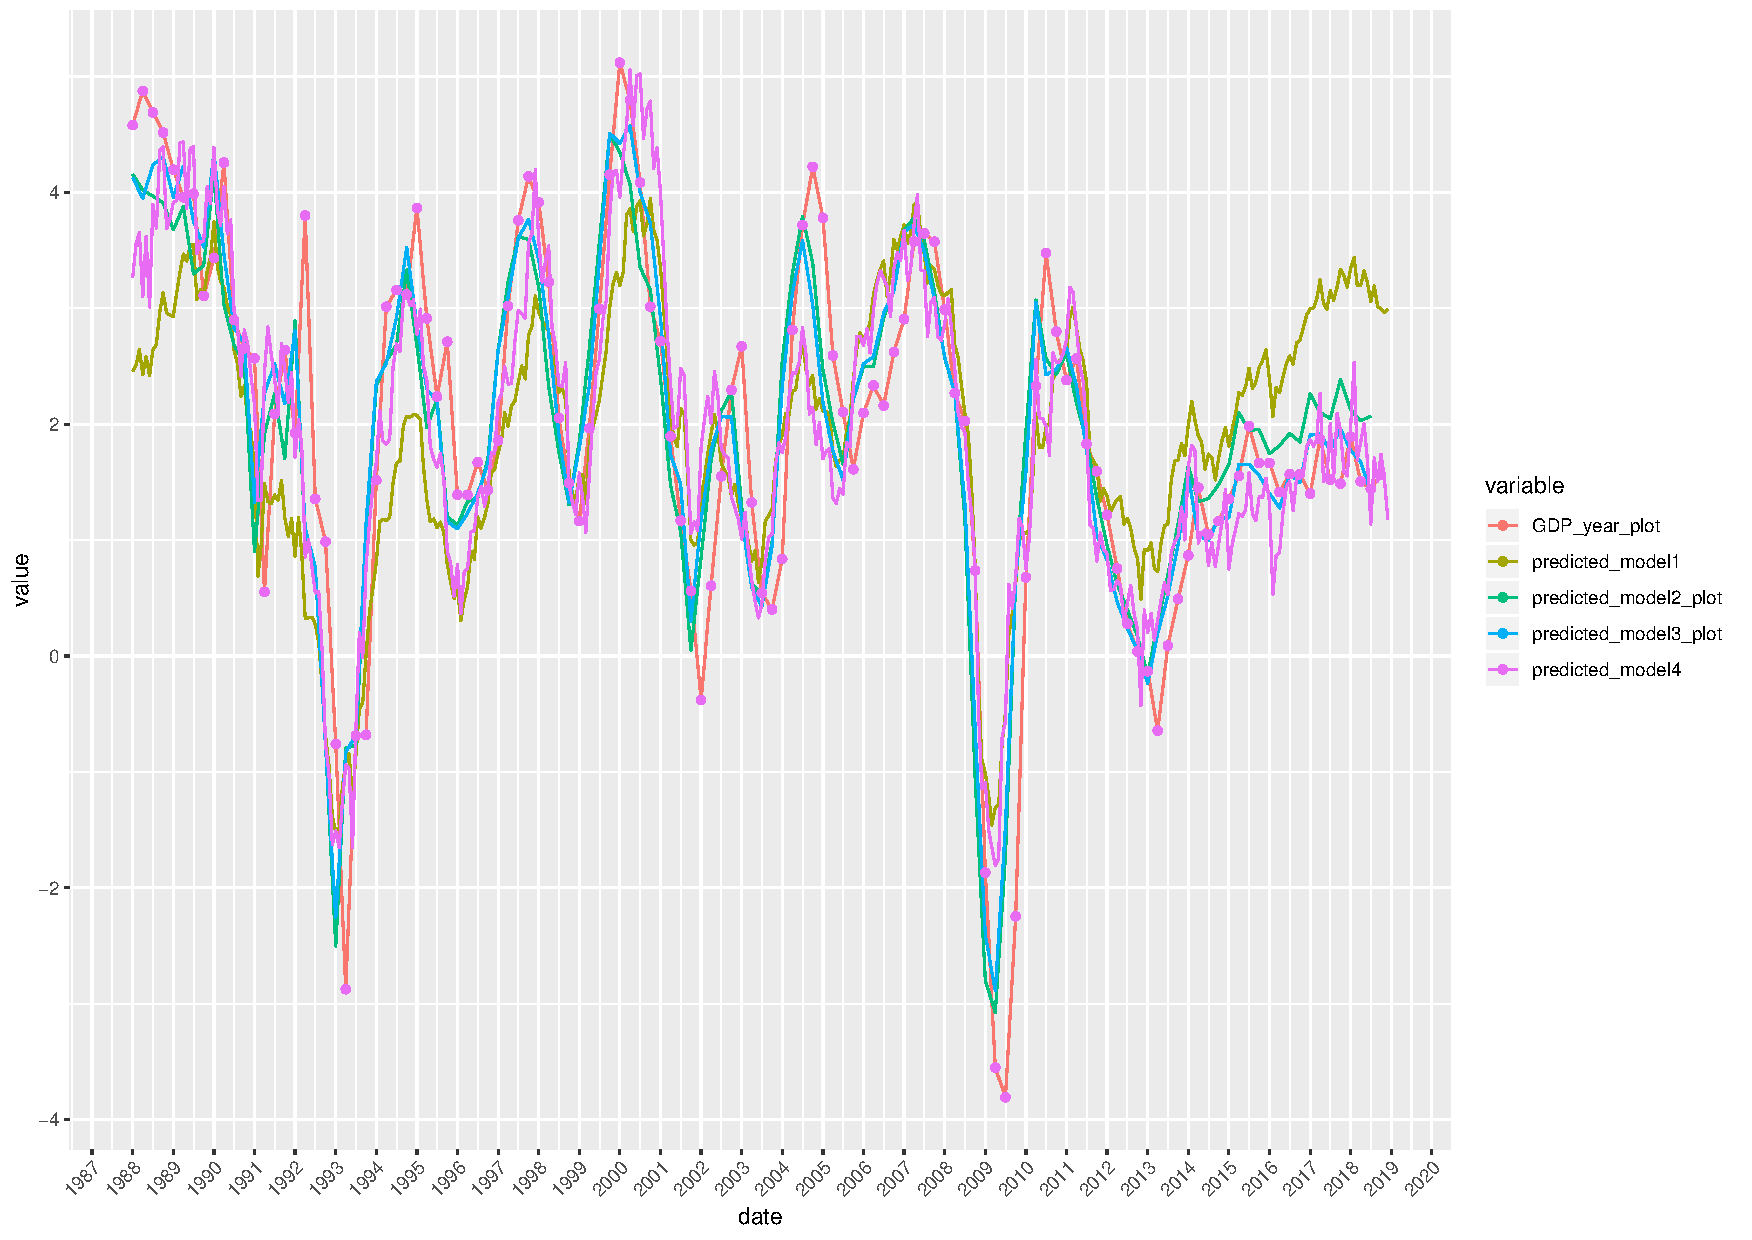
\includegraphics[scale=0.5]{Graphs/pred1.pdf}
    \caption{Plot }
    \label{fig:pred1}
\end{figure}



\begin{table}[H] \centering 
%  \caption{} 
%  \label{} 
\begin{tabular}{@{\extracolsep{5pt}}lD{.}{.}{-3} D{.}{.}{-3} D{.}{.}{-3} D{.}{.}{-3} } 
\\[-1.8ex] & \multicolumn{4}{c}{GDP\_year} \\ 
\\[-1.8ex] & \multicolumn{1}{c}{(1)} & \multicolumn{1}{c}{(2)} & \multicolumn{1}{c}{(3)} & \multicolumn{1}{c}{(4)}\\ 
\hline \\[-1.8ex] 
 Constant & 3.364^{***} & -4.052^{***} & -3.993^{***} & -0.985 \\ 
  & (0.173) & (0.922) & (0.917) & (0.797) \\ 
  &&&& \\ 
 E\_I & 14.491^{***} & 22.080^{***} & 21.579^{***} & 5.629^{***} \\ 
  & (1.390) & (1.392) & (1.421) & (2.091) \\ 
  &&&& \\ 
 E\_I\_diff & 11.538^{*} &  & 8.181 & 24.063^{***} \\ 
  & (6.560) &  & (5.309) & (4.488) \\ 
  &&&& \\ 
 Var\_I &  & 27.506^{***} & 27.105^{***} & 7.179^{**} \\ 
  &  & (3.349) & (3.340) & (3.433) \\ 
  &&&& \\ 
 GDP\_year\_lag1 &  &  &  & 0.687^{***} \\ 
  &  &  &  & (0.076) \\ 
  &&&& \\ 
\hline \\[-1.8ex] 
R$^{2}$ & \multicolumn{1}{c}{0.512} & \multicolumn{1}{c}{0.679} & \multicolumn{1}{c}{0.685} & \multicolumn{1}{c}{0.813} \\ 
Adjusted R$^{2}$ & \multicolumn{1}{c}{0.504} & \multicolumn{1}{c}{0.673} & \multicolumn{1}{c}{0.677} & \multicolumn{1}{c}{0.806} \\ 
Residual Std. Error & \multicolumn{1}{c}{1.162} & \multicolumn{1}{c}{0.943} & \multicolumn{1}{c}{0.938} & \multicolumn{1}{c}{0.729} \\ 
F Statistic & \multicolumn{1}{c}{63.468$^{***}$} & \multicolumn{1}{c}{127.781$^{***}$} & \multicolumn{1}{c}{86.947$^{***}$} & \multicolumn{1}{c}{128.113$^{***}$} \\
\end{tabular} 
\end{table} 

\begin{figure}[H]
    \centering
    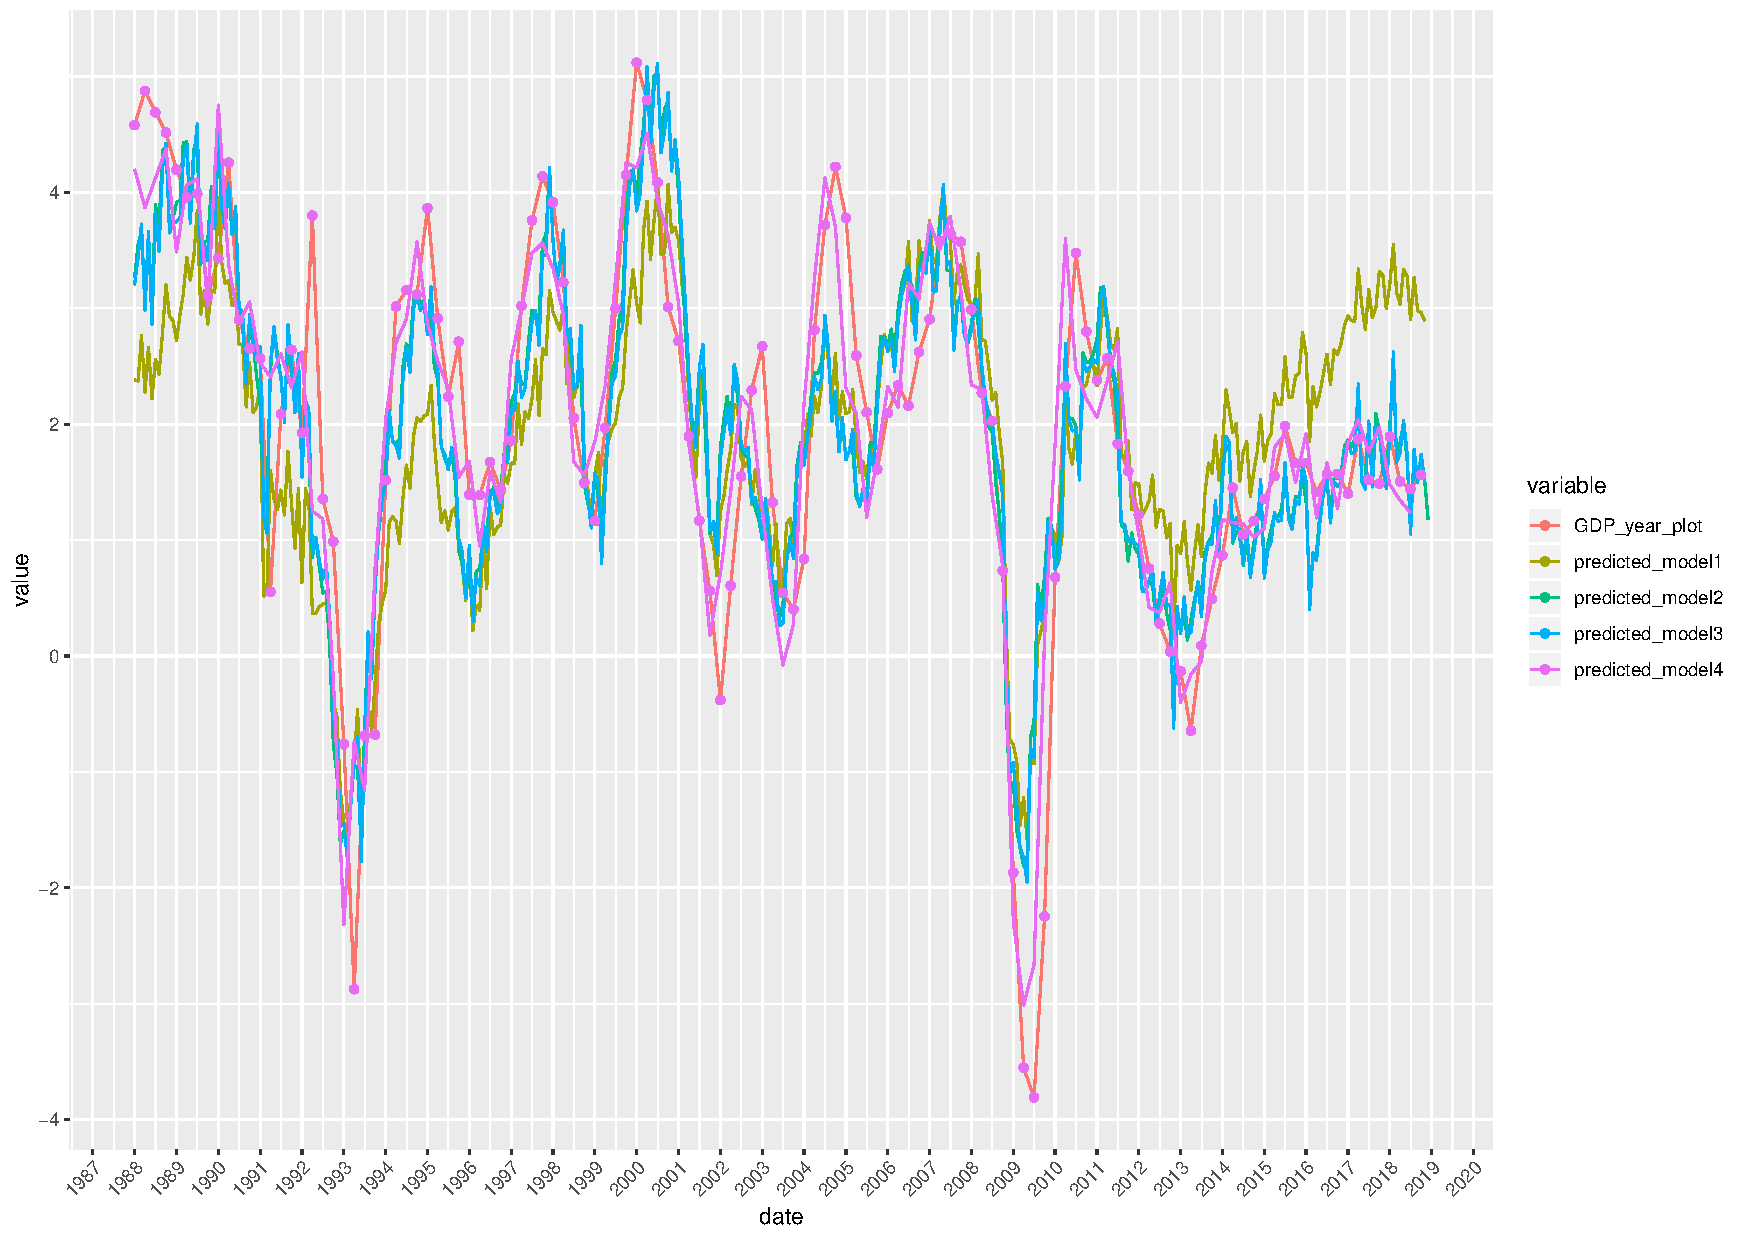
\includegraphics[scale=0.5]{Graphs/pred2.pdf}
    \caption{Plot }
    \label{pred2}
\end{figure}

\begin{eqnarray}
    \Var \left(\frac{X_{Q1} + X_{Q2} + X_{Q3} + X_{Q4}}{4} \right) &=& \frac{1}{16} \large[ \Var(X_{Q1}) + \Var(X_{Q2}) + \Var(X_{Q3}) + \Var(X_{Q4}) \nonumber \\
    && + \Cov (X_{Q1},X_{Q2}) + \Cov (X_{Q1},X_{Q3}) + \Cov (X_{Q1},X_{Q4}) \nonumber \\
    &&  + \Cov (X_{Q2},X_{Q3}) + \Cov (X_{Q2},X_{Q4}) + \Cov (X_{Q3},X_{Q4}) \large] \nonumber
\end{eqnarray}

\begin{eqnarray}
    \Var \left(\frac{X_{Q1} + X_{Q2} + \ldots + X_{Qn}}{n} \right) 
    &=& \Var \left(\frac{\pi_{1+} + \pi_{2+} + \ldots + \pi_{n+} - \pi_{1-} - \pi_{2-} - \ldots - \pi_{n-} }{n} \right) \nonumber \\
    &=& \frac{1}{n^2} \Var \left(\pi_{1+} + \pi_{2+} + \ldots + \pi_{n+} - \pi_{1-} - \pi_{2-} - \ldots - \pi_{n-} \right) \nonumber \\
\end{eqnarray}




\section{Discussion regarding the 'true variance'}

There is another way to calculate the variance that have been ignored; the calculation of the variance for each lowest group of globalisation, and then combine those calculated variances.

Interestingly, it have been calculated for several questions of the business barometer, and it is approximately 10 times smaller than the variance based on all the answer a ones.

The reasons why it will not be used here
- losing information
- weight of globalisation taken into account in the weighted variance





\newpage

\begin{table}[!htbp] \centering 
%  \caption{} 
%  \label{} 
\begin{tabular}{@{\extracolsep{5pt}}lD{.}{.}{-3} D{.}{.}{-3} } 
\\[-1.8ex] & \multicolumn{2}{c}{GDP\_year} \\ 
\\[-1.8ex] & \multicolumn{1}{c}{(1)} & \multicolumn{1}{c}{(2)}\\ 
\hline \\[-1.8ex] 
 E\_I & 22.783^{***} & 23.088^{***} \\ 
  & (1.340) & (1.319) \\ 
  & & \\ 
 Var\_I & 22.151^{***} & 28.508^{***} \\ 
  & (6.050) & (3.133) \\ 
  & & \\ 
 Z\_I & -24.279^{***} & -25.008^{***} \\ 
  & (5.765) & (5.746) \\ 
  & & \\ 
 Var\_Z\_I & 6.609 &  \\ 
  & (5.383) &  \\ 
  & & \\ 
 Constant & -4.090^{***} & -4.265^{***} \\ 
  & (0.871) & (0.861) \\ 
  & & \\ 
\hline \\[-1.8ex] 
R$^{2}$ & \multicolumn{1}{c}{0.726} & \multicolumn{1}{c}{0.722} \\ 
Adjusted R$^{2}$ & \multicolumn{1}{c}{0.717} & \multicolumn{1}{c}{0.716} \\ 
Residual Std. Error & \multicolumn{1}{c}{0.878 (df = 119)} & \multicolumn{1}{c}{0.880 (df = 120)} \\ 
F Statistic & \multicolumn{1}{c}{78.806$^{***}$ (df = 4; 119)} & \multicolumn{1}{c}{104.133$^{***}$ (df = 3; 120)} \\ 

\end{tabular} 
\end{table} 

\begin{figure}[H]
    \centering
    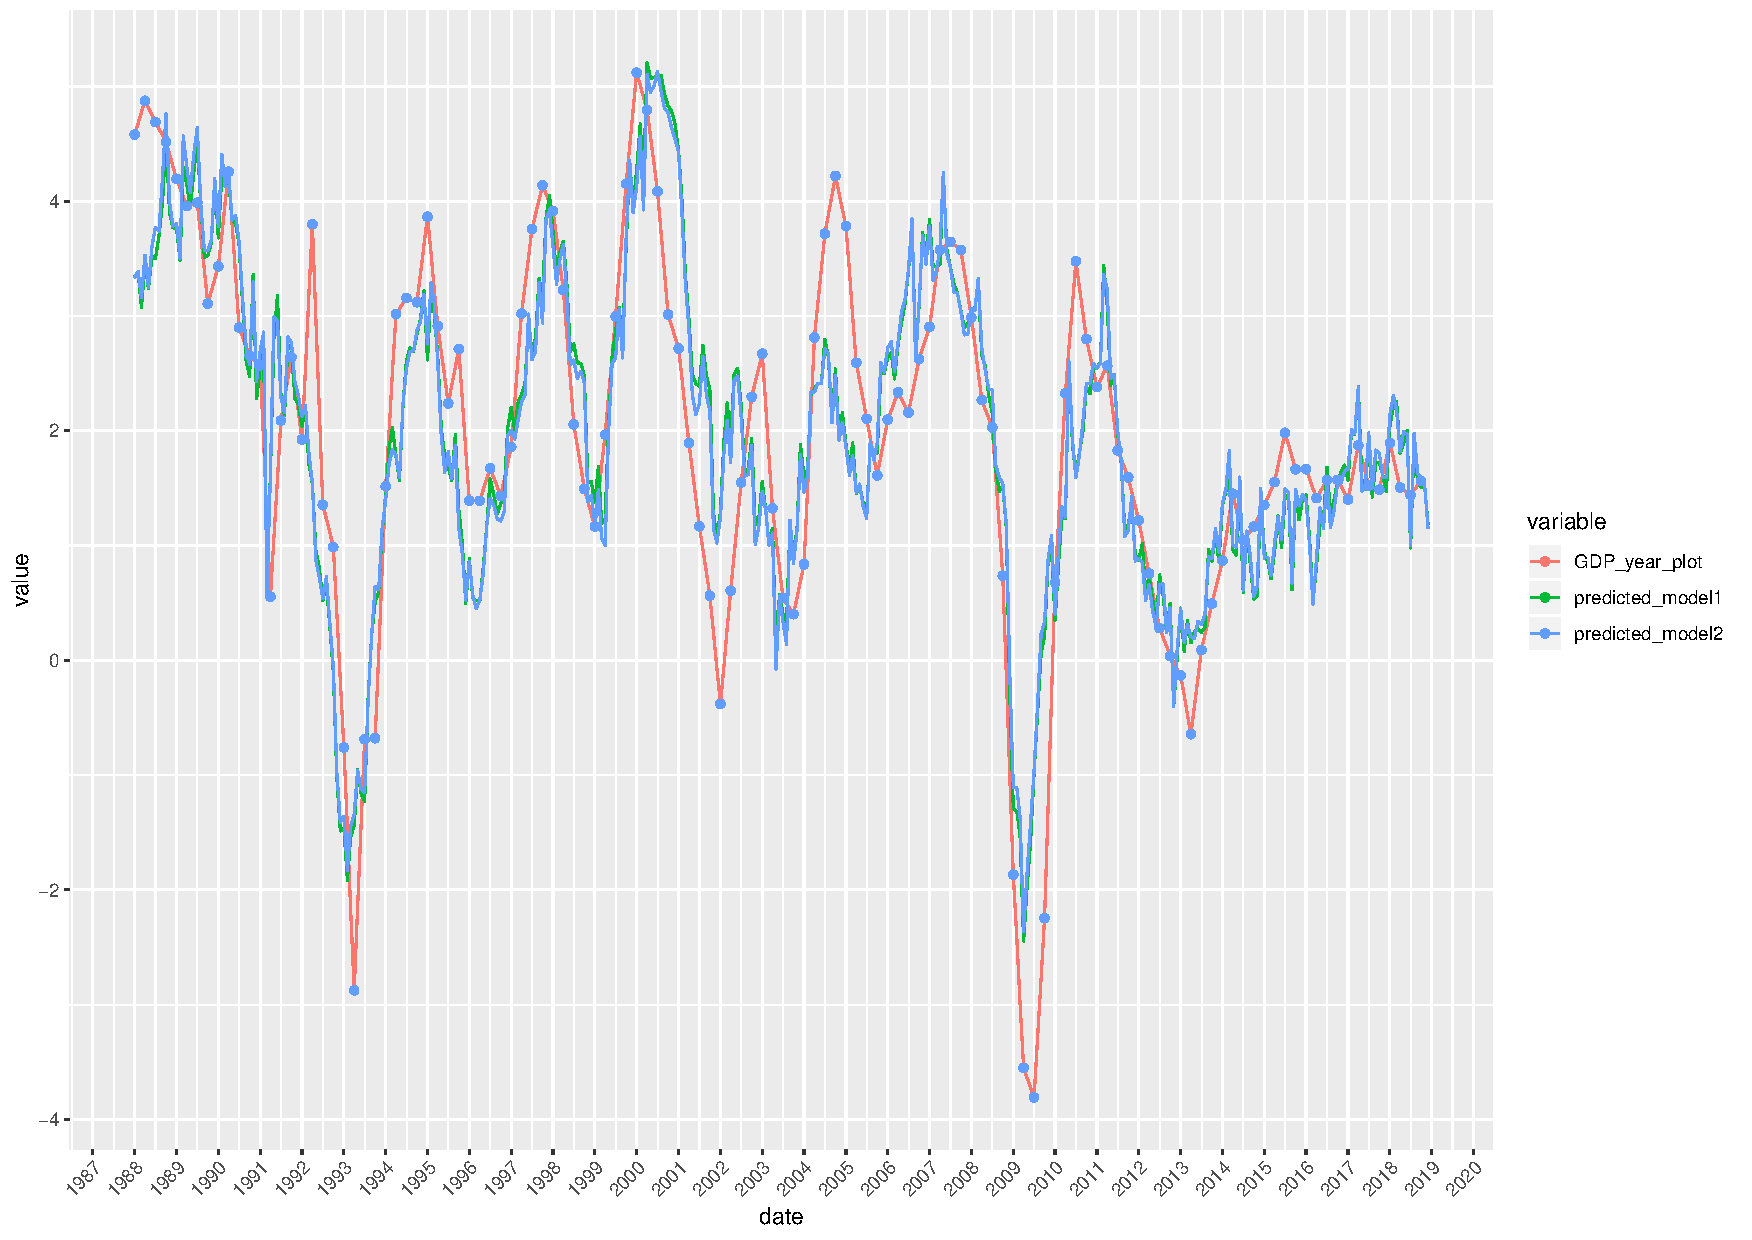
\includegraphics[scale=0.5]{Graphs/pred3.pdf}
    \caption{Plot }
    \label{pred3}
\end{figure}









\begin{center}
\begin{tabular}{r | r | r | r | c c c | }
 \multicolumn{3}{r}{} & \multicolumn{1}{r}{} &	\multicolumn{3}{c}{$t$} \\ \cline{5-7}
 \multicolumn{3}{r}{} & 		& \textbf{-} & \textbf{0} & \textbf{+} \\ \cline{2-2} \cline{4-7}
&&& \textbf{-} & $\pi_{---}$ & $\pi_{--0}$ & $\pi_{--+}$ \\ 
&  $-$ &$t-1$ & \textbf{0} & $\pi_{-0-}$	& $\pi_{-00}$ & $\pi_{-0+}$	\\
&&&\textbf{+} & $\pi_{-+-}$	& $\pi_{-+0}$	& $\pi_{-++}$ \\ \cline{2-2} \cline{4-7}
&&&\textbf{-} & $\pi_{0--}$	& $\pi_{0-0}$	& $\pi_{0-+}$ \\ 
$t-2$ & $0$   &$t-1$ & \textbf{0} & $\pi_{00-}$	& $\pi_{000}$	& $\pi_{00+}$	\\
&&&\textbf{+} & $\pi_{0+-}$	& $\pi_{0+0}$	& $\pi_{0++}$ \\ \cline{2-2} \cline{4-7}
&&&\textbf{-} & $\pi_{+--}$	& $\pi_{+-0}$	& $\pi_{+-+}$ \\ 
&$+$   &$t-1$ & \textbf{0} & $\pi_{+0-}$	& $\pi_{+00}$	& $\pi_{+0+}$	\\
&&&\textbf{+} & $\pi_{++-}$	& $\pi_{++0}$	& $\pi_{+++}$ \\ \cline{2-2} \cline{4-7}
		
\end{tabular}    
\end{center}

\begin{center}
\begin{tabular}{r | r | r | r | c c c | }
 \multicolumn{3}{r}{} & \multicolumn{1}{r}{} &	\multicolumn{3}{c}{$t$} \\ \cline{5-7}
 \multicolumn{3}{r}{} & 		& \textbf{-} & \textbf{0} & \textbf{+} \\ \cline{2-2} \cline{4-7}
&&& \textbf{-}              & $\pi_{---}=0$ & $\pi_{--0}=2$ & $\pi_{--+}=3$ \\ 
&$-$ &$t-1$&\textbf{0}      & $\pi_{-0-}=0$	& $\pi_{-00}=1$ & $\pi_{-0+}=2$	\\
&&&\textbf{+}               & $\pi_{-+-}=-1$& $\pi_{-+0}=0$	& $\pi_{-++}=1$ \\ \cline{2-2} \cline{4-7}
&&&\textbf{-}               & $\pi_{0--}=-1$	& $\pi_{0-0}=1$	    & $\pi_{0-+}=2$ \\ 
$t-2$&$0$&$t-1$&\textbf{0}  & $\pi_{00-}=-1$	& $\pi_{000}=0$	    & $\pi_{00+}=1$	\\
&&&\textbf{+}               & $\pi_{0+-}=-2$	& $\pi_{0+0}=-1$    & $\pi_{0++}=0$ \\ \cline{2-2} \cline{4-7}
&&&\textbf{-}               & $\pi_{+--}=-1$	& $\pi_{+-0}=0$	    & $\pi_{+-+}=1$ \\ 
&$+$   &$t-1$ & \textbf{0}  & $\pi_{+0-}=-2$	& $\pi_{+00}=-1$    & $\pi_{+0+}=0$	\\
&&&\textbf{+}               & $\pi_{++-}=-3$	& $\pi_{++0}=-2$    & $\pi_{+++}=0$ \\ \cline{2-2} \cline{4-7}
		
\end{tabular}    
\end{center}



\begin{center}
\begin{tabular}{r | r | r | r | c c c | }
 \multicolumn{3}{r}{} & \multicolumn{1}{r}{} &	\multicolumn{3}{c}{$t$} \\ \cline{5-7}
 \multicolumn{3}{r}{} & 		& \textbf{-} & \textbf{0} & \textbf{+} \\ \cline{2-2} \cline{4-7}
&&& \textbf{-}              & $0$	& $2$	& $3$ \\ 
& $-$ &$t-1$ & \textbf{0}   & $0$	& $1$	& $2$	\\
&&& \textbf{+}              & $-1$ & $0$	& $1$ \\ \cline{2-2} \cline{4-7}
&&& \textbf{-}              & $-1$ & $1$	& $2$ \\ 
$t-2$&$0$&$t-1$&\textbf{0}  & $-1$	& $0$	& $1$	\\
&&&    \textbf{+}           & $-2$ & $-1$	& $1$ \\ \cline{2-2} \cline{4-7}
&&&    \textbf{-}           & $-1$ & $0$	& $1$ \\ 
&$+$   &$t-1$ & \textbf{0}  & $-2$	& $-1$	& $0$	\\
&&& \textbf{+}              & $-3$	& $-2$	& $0$ \\ \cline{2-2} \cline{4-7}
\end{tabular}    
\end{center}



\end{document}